\chapter{RRT}\label{chap:RRT}

\section{General}

The goal of this Thesis was not only to generate a numerical stable, snap optimized polynomial trajectory but also to explore a dense (indoor) environment and plan an aggressive trajectory in between the obstacles. Hence, the Rapidly-Exploring Random Tree (RRT) algorithm is used to find a collision free straight-line solution through the dense environment. The sampling points oft the RRT (or RRT*) algorithm are then used as the vertices in the polynomial optimization.

\section{Algorithm}

\subsection{RRT}

\subsection{RRT*}



\begin{figure}[h]
   \centering
   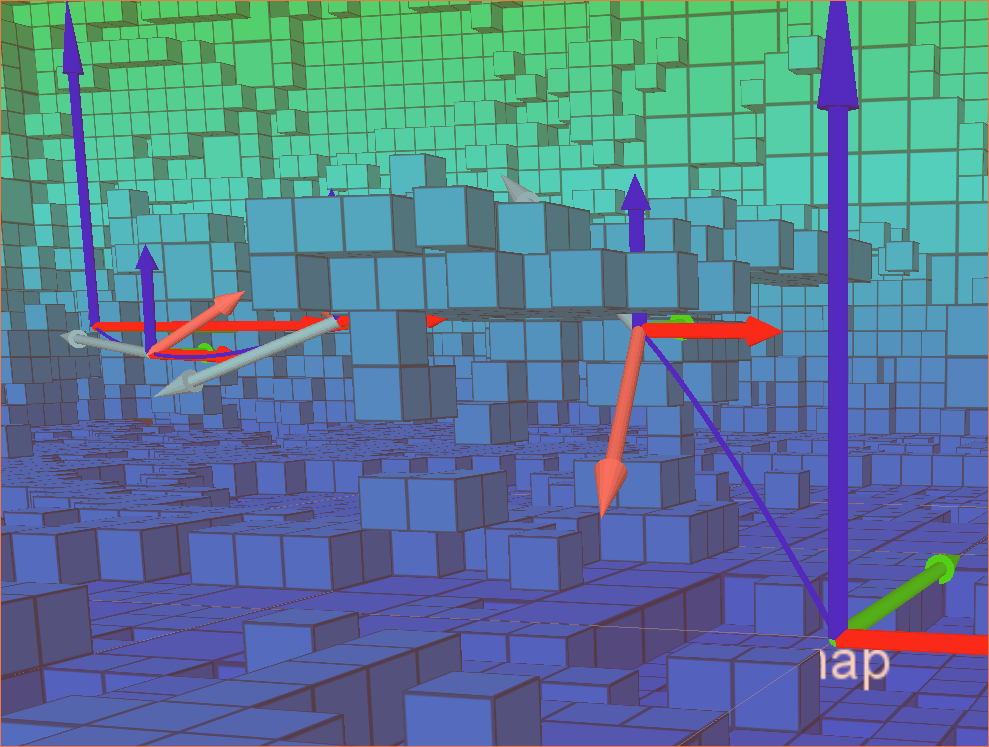
\includegraphics[width=1\textwidth]{pics/initialSolution.png}
   \caption{Ein Bild.}
\end{figure}


\begin{figure}[h]
   \centering
   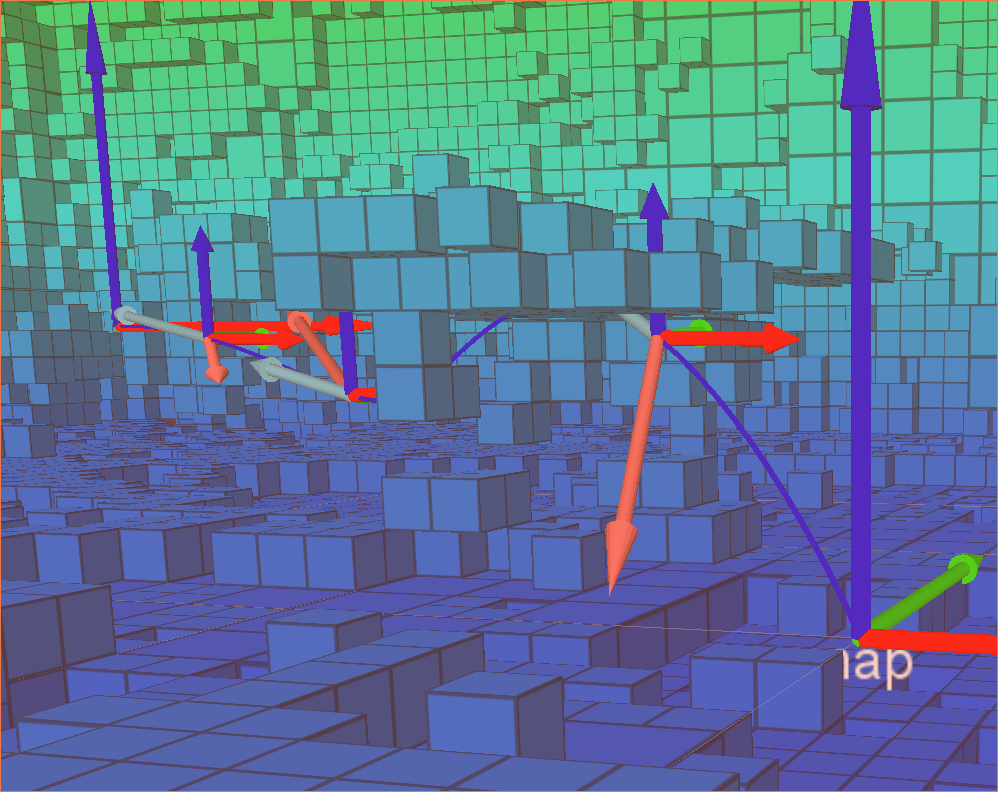
\includegraphics[width=1\textwidth]{pics/Vertex_in_middle_2.png}
   \caption{Ein Bild.}
\end{figure}

\begin{figure}[h]
   \centering
   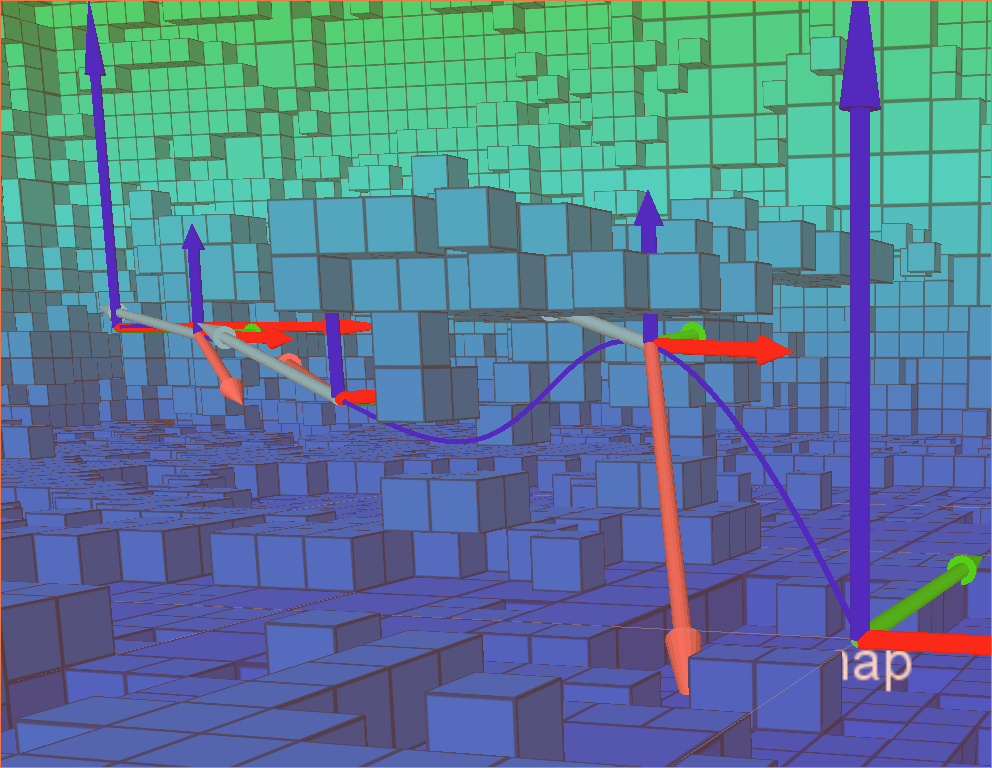
\includegraphics[width=1\textwidth]{pics/section.png}
   \caption{Ein Bild.}
\end{figure}



\begin{figure}[h]
   \centering
   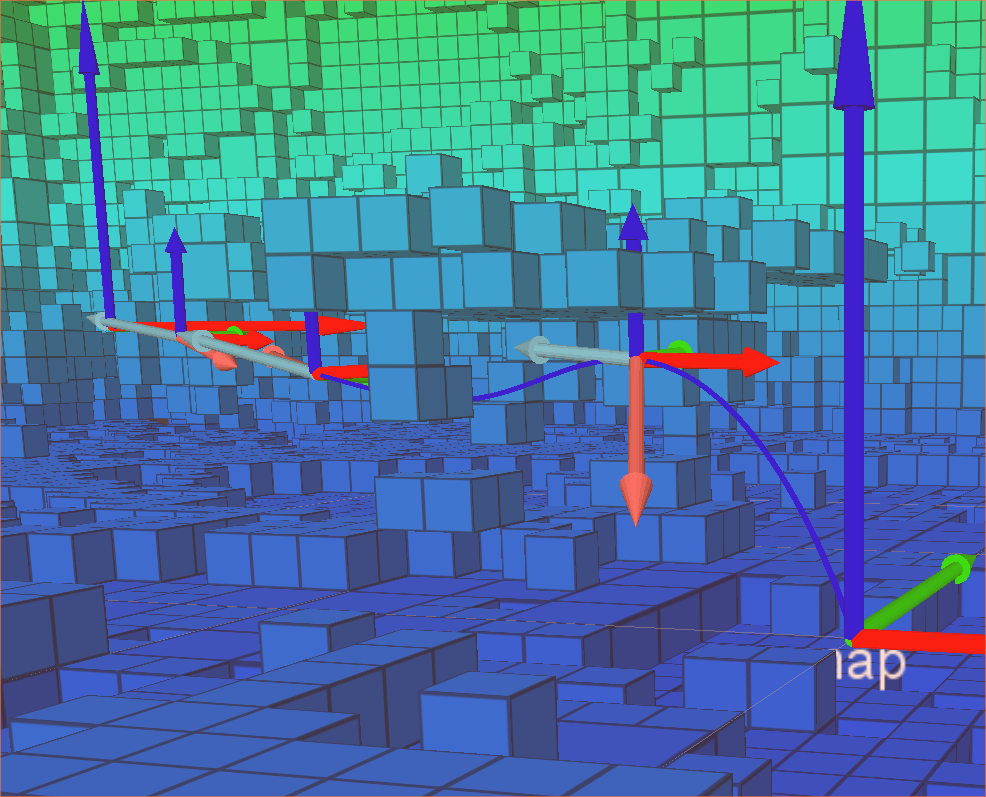
\includegraphics[width=1\textwidth]{pics/section_and_time.png}
   \caption{Ein Bild.}
\end{figure}


\begin{figure}[h]
   \centering
   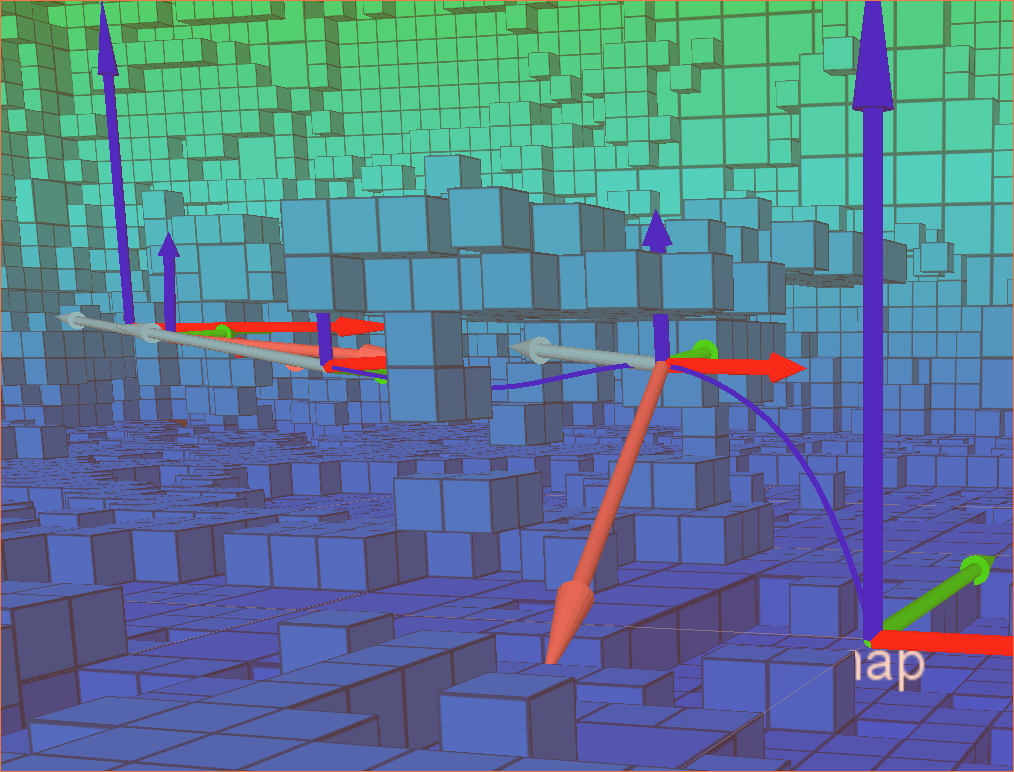
\includegraphics[width=1\textwidth]{pics/Nlopt_after_sectionAndTime.png}
   \caption{Ein Bild.}
\end{figure}